% Options for packages loaded elsewhere
\PassOptionsToPackage{unicode}{hyperref}
\PassOptionsToPackage{hyphens}{url}
%
\documentclass[
]{book}
\title{Time Series Memories (always in construction)}
\author{María José Olmo Uceda}
\date{2022-04-19}

\usepackage{amsmath,amssymb}
\usepackage{lmodern}
\usepackage{iftex}
\ifPDFTeX
  \usepackage[T1]{fontenc}
  \usepackage[utf8]{inputenc}
  \usepackage{textcomp} % provide euro and other symbols
\else % if luatex or xetex
  \usepackage{unicode-math}
  \defaultfontfeatures{Scale=MatchLowercase}
  \defaultfontfeatures[\rmfamily]{Ligatures=TeX,Scale=1}
\fi
% Use upquote if available, for straight quotes in verbatim environments
\IfFileExists{upquote.sty}{\usepackage{upquote}}{}
\IfFileExists{microtype.sty}{% use microtype if available
  \usepackage[]{microtype}
  \UseMicrotypeSet[protrusion]{basicmath} % disable protrusion for tt fonts
}{}
\makeatletter
\@ifundefined{KOMAClassName}{% if non-KOMA class
  \IfFileExists{parskip.sty}{%
    \usepackage{parskip}
  }{% else
    \setlength{\parindent}{0pt}
    \setlength{\parskip}{6pt plus 2pt minus 1pt}}
}{% if KOMA class
  \KOMAoptions{parskip=half}}
\makeatother
\usepackage{xcolor}
\IfFileExists{xurl.sty}{\usepackage{xurl}}{} % add URL line breaks if available
\IfFileExists{bookmark.sty}{\usepackage{bookmark}}{\usepackage{hyperref}}
\hypersetup{
  pdftitle={Time Series Memories (always in construction)},
  pdfauthor={María José Olmo Uceda},
  hidelinks,
  pdfcreator={LaTeX via pandoc}}
\urlstyle{same} % disable monospaced font for URLs
\usepackage{color}
\usepackage{fancyvrb}
\newcommand{\VerbBar}{|}
\newcommand{\VERB}{\Verb[commandchars=\\\{\}]}
\DefineVerbatimEnvironment{Highlighting}{Verbatim}{commandchars=\\\{\}}
% Add ',fontsize=\small' for more characters per line
\usepackage{framed}
\definecolor{shadecolor}{RGB}{248,248,248}
\newenvironment{Shaded}{\begin{snugshade}}{\end{snugshade}}
\newcommand{\AlertTok}[1]{\textcolor[rgb]{0.94,0.16,0.16}{#1}}
\newcommand{\AnnotationTok}[1]{\textcolor[rgb]{0.56,0.35,0.01}{\textbf{\textit{#1}}}}
\newcommand{\AttributeTok}[1]{\textcolor[rgb]{0.77,0.63,0.00}{#1}}
\newcommand{\BaseNTok}[1]{\textcolor[rgb]{0.00,0.00,0.81}{#1}}
\newcommand{\BuiltInTok}[1]{#1}
\newcommand{\CharTok}[1]{\textcolor[rgb]{0.31,0.60,0.02}{#1}}
\newcommand{\CommentTok}[1]{\textcolor[rgb]{0.56,0.35,0.01}{\textit{#1}}}
\newcommand{\CommentVarTok}[1]{\textcolor[rgb]{0.56,0.35,0.01}{\textbf{\textit{#1}}}}
\newcommand{\ConstantTok}[1]{\textcolor[rgb]{0.00,0.00,0.00}{#1}}
\newcommand{\ControlFlowTok}[1]{\textcolor[rgb]{0.13,0.29,0.53}{\textbf{#1}}}
\newcommand{\DataTypeTok}[1]{\textcolor[rgb]{0.13,0.29,0.53}{#1}}
\newcommand{\DecValTok}[1]{\textcolor[rgb]{0.00,0.00,0.81}{#1}}
\newcommand{\DocumentationTok}[1]{\textcolor[rgb]{0.56,0.35,0.01}{\textbf{\textit{#1}}}}
\newcommand{\ErrorTok}[1]{\textcolor[rgb]{0.64,0.00,0.00}{\textbf{#1}}}
\newcommand{\ExtensionTok}[1]{#1}
\newcommand{\FloatTok}[1]{\textcolor[rgb]{0.00,0.00,0.81}{#1}}
\newcommand{\FunctionTok}[1]{\textcolor[rgb]{0.00,0.00,0.00}{#1}}
\newcommand{\ImportTok}[1]{#1}
\newcommand{\InformationTok}[1]{\textcolor[rgb]{0.56,0.35,0.01}{\textbf{\textit{#1}}}}
\newcommand{\KeywordTok}[1]{\textcolor[rgb]{0.13,0.29,0.53}{\textbf{#1}}}
\newcommand{\NormalTok}[1]{#1}
\newcommand{\OperatorTok}[1]{\textcolor[rgb]{0.81,0.36,0.00}{\textbf{#1}}}
\newcommand{\OtherTok}[1]{\textcolor[rgb]{0.56,0.35,0.01}{#1}}
\newcommand{\PreprocessorTok}[1]{\textcolor[rgb]{0.56,0.35,0.01}{\textit{#1}}}
\newcommand{\RegionMarkerTok}[1]{#1}
\newcommand{\SpecialCharTok}[1]{\textcolor[rgb]{0.00,0.00,0.00}{#1}}
\newcommand{\SpecialStringTok}[1]{\textcolor[rgb]{0.31,0.60,0.02}{#1}}
\newcommand{\StringTok}[1]{\textcolor[rgb]{0.31,0.60,0.02}{#1}}
\newcommand{\VariableTok}[1]{\textcolor[rgb]{0.00,0.00,0.00}{#1}}
\newcommand{\VerbatimStringTok}[1]{\textcolor[rgb]{0.31,0.60,0.02}{#1}}
\newcommand{\WarningTok}[1]{\textcolor[rgb]{0.56,0.35,0.01}{\textbf{\textit{#1}}}}
\usepackage{longtable,booktabs,array}
\usepackage{calc} % for calculating minipage widths
% Correct order of tables after \paragraph or \subparagraph
\usepackage{etoolbox}
\makeatletter
\patchcmd\longtable{\par}{\if@noskipsec\mbox{}\fi\par}{}{}
\makeatother
% Allow footnotes in longtable head/foot
\IfFileExists{footnotehyper.sty}{\usepackage{footnotehyper}}{\usepackage{footnote}}
\makesavenoteenv{longtable}
\usepackage{graphicx}
\makeatletter
\def\maxwidth{\ifdim\Gin@nat@width>\linewidth\linewidth\else\Gin@nat@width\fi}
\def\maxheight{\ifdim\Gin@nat@height>\textheight\textheight\else\Gin@nat@height\fi}
\makeatother
% Scale images if necessary, so that they will not overflow the page
% margins by default, and it is still possible to overwrite the defaults
% using explicit options in \includegraphics[width, height, ...]{}
\setkeys{Gin}{width=\maxwidth,height=\maxheight,keepaspectratio}
% Set default figure placement to htbp
\makeatletter
\def\fps@figure{htbp}
\makeatother
\setlength{\emergencystretch}{3em} % prevent overfull lines
\providecommand{\tightlist}{%
  \setlength{\itemsep}{0pt}\setlength{\parskip}{0pt}}
\setcounter{secnumdepth}{5}
\usepackage{booktabs}
\ifLuaTeX
  \usepackage{selnolig}  % disable illegal ligatures
\fi
\usepackage[]{natbib}
\bibliographystyle{plainnat}

\begin{document}
\maketitle

{
\setcounter{tocdepth}{1}
\tableofcontents
}
\hypertarget{introduction}{%
\chapter{Introduction}\label{introduction}}

Analysis of gene expression data in time series of viral infections. Tracking of the selected experiments and the processes followed from data download to DEG.

One the differently expressed genes have been selected we will beging the study of those genes that can serve as early warnings. The first method we use use is based on \textbf{Dynamical Network Biomarkers}.

\hypertarget{general-workflow}{%
\section{General workflow}\label{general-workflow}}

\begin{figure}
\centering
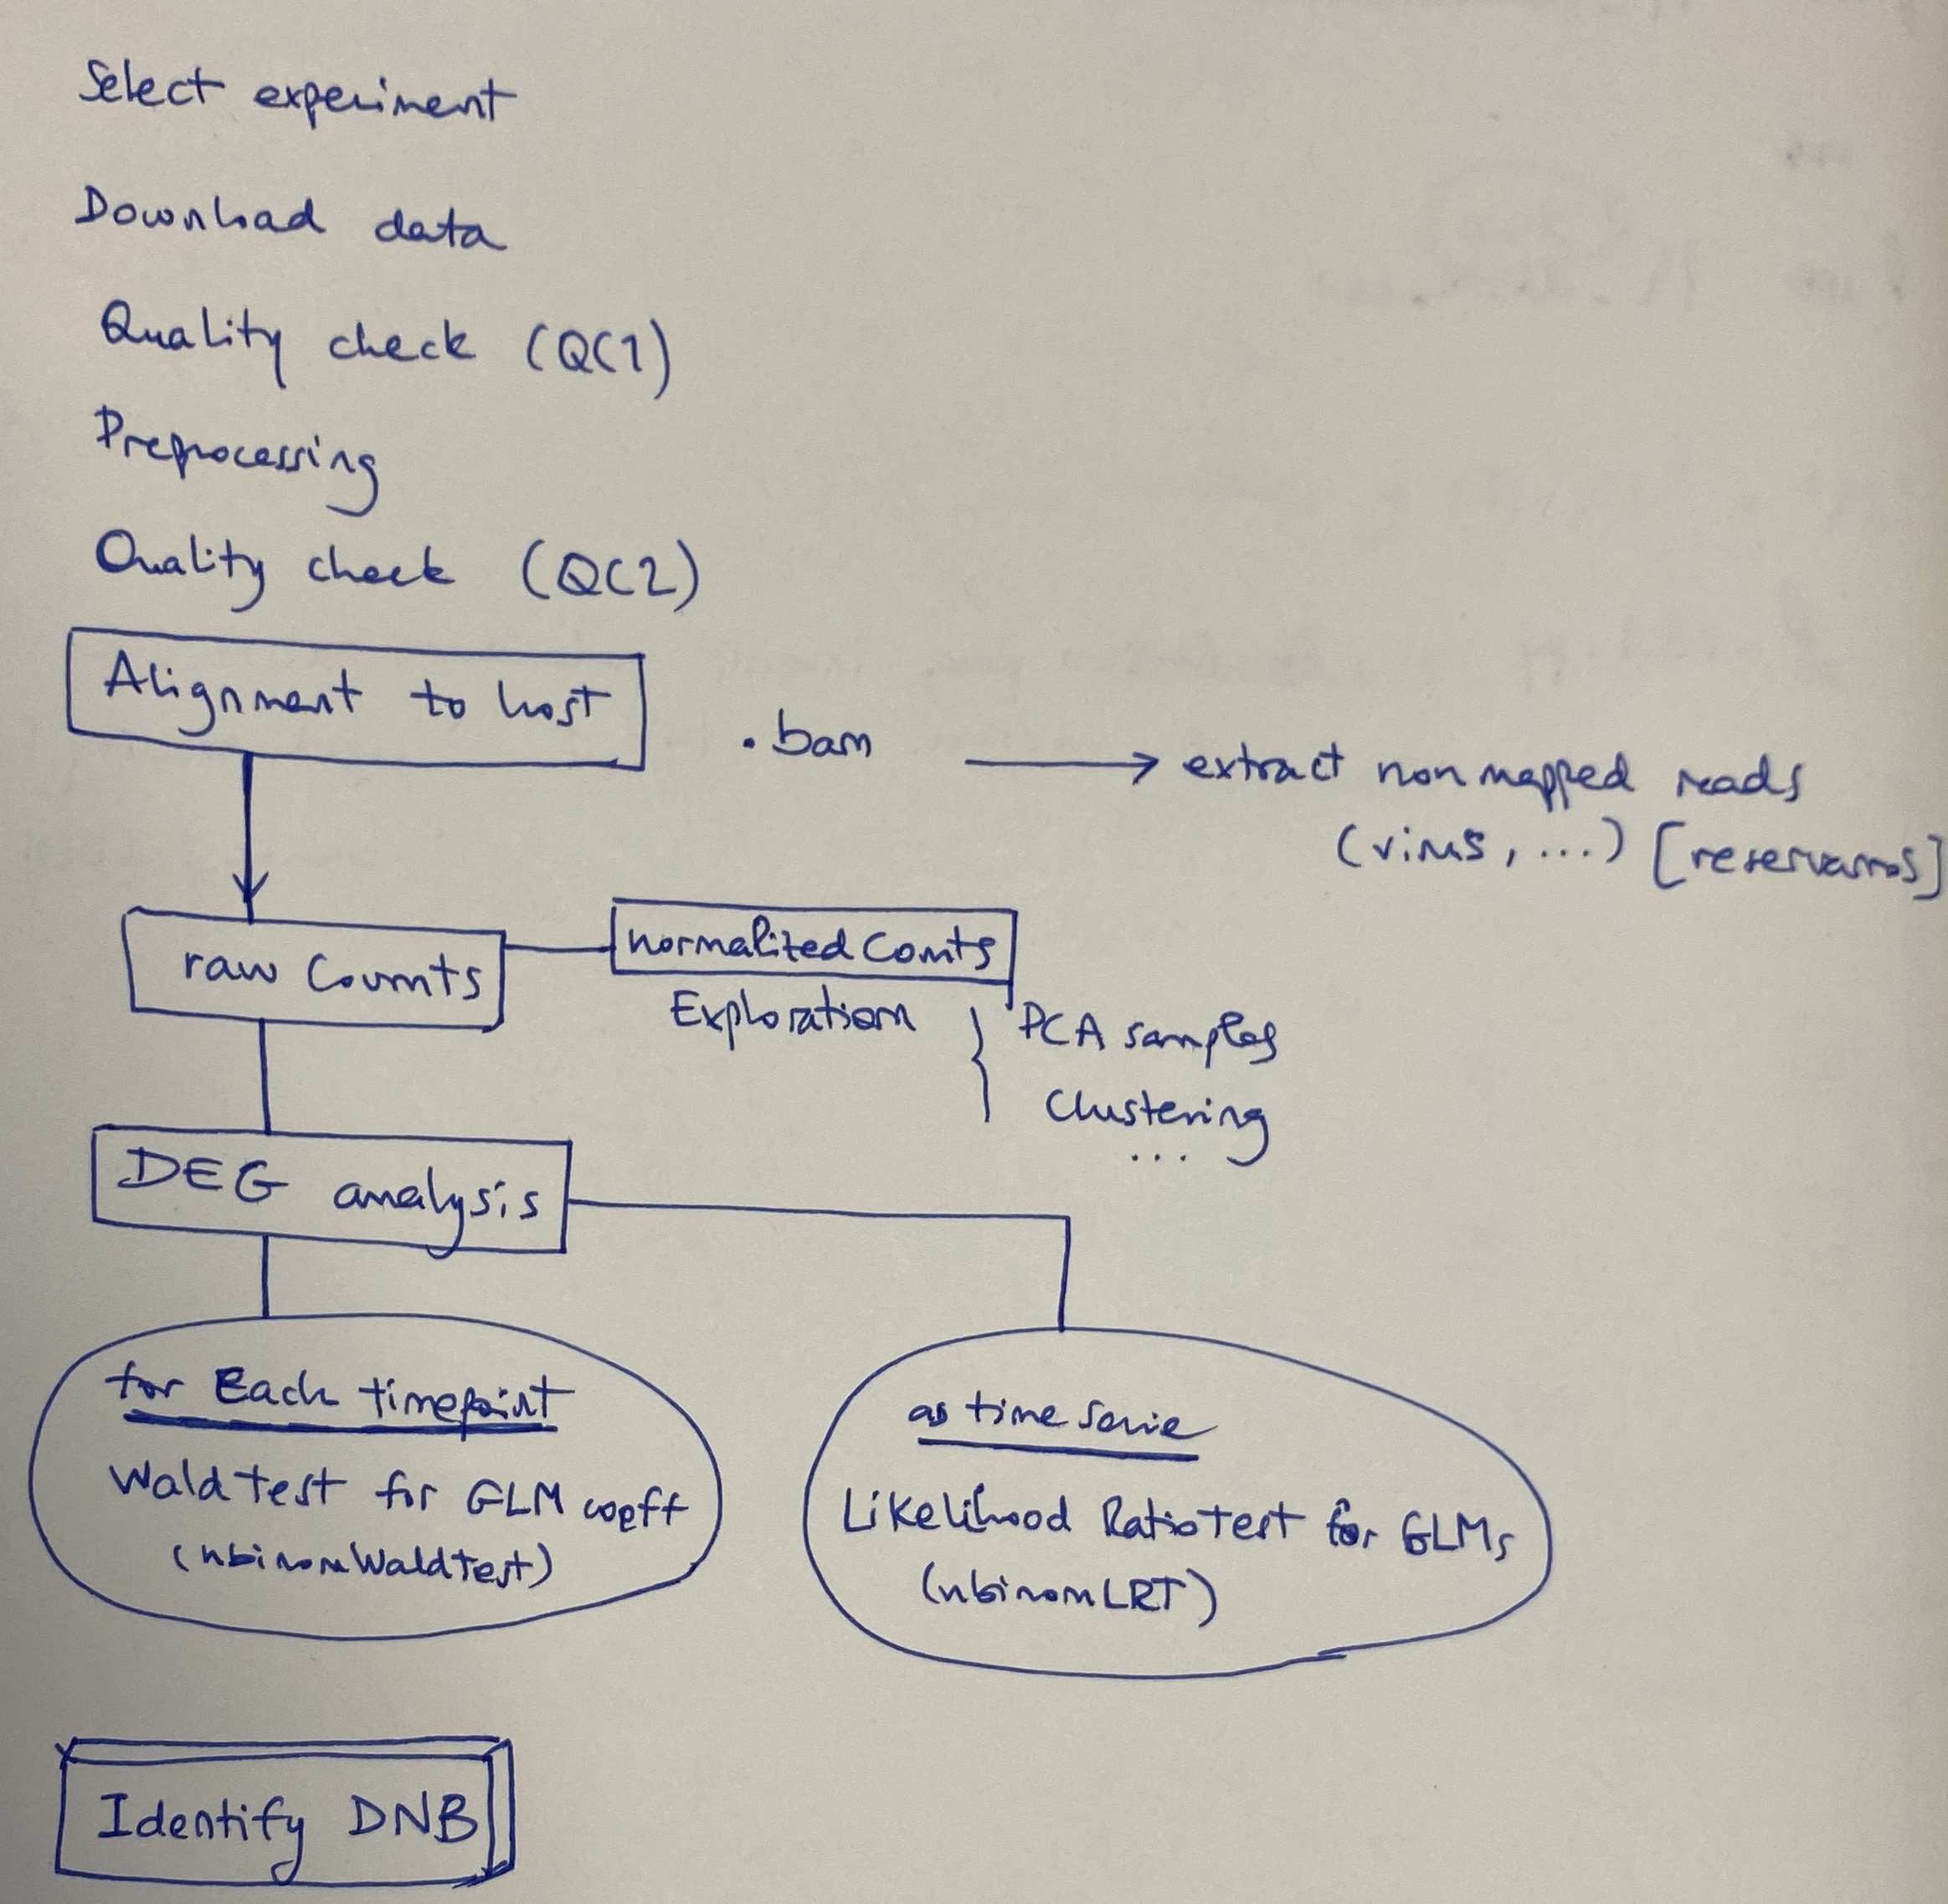
\includegraphics{images/general_workflow.jpg}
\caption{General process}
\end{figure}

General information:

\begin{itemize}
\tightlist
\item
  From begining to matrix counts: \protect\hyperlink{previous-steps}{chapter 3}\\
\item
  DEG analysis: \protect\hyperlink{deg-analysis}{chapter 4}
\end{itemize}

Each project analyzed will have its own chapter

\hypertarget{experiments}{%
\chapter{Experiments selected}\label{experiments}}

Previous conditions:

\begin{itemize}
\tightlist
\item
  Viral infection time series data available\\
\item
  At least 4 time points\\
\item
  Control non infected for each time point\\
\item
  Preferably RNA-seq but we will study the microarray data previously selected by Juan Carlos and Santiago.
\end{itemize}

I will start by the RNA-seq data, and adding the datasets following the chronology of their analysis.

\hypertarget{public-data}{%
\section{Public data}\label{public-data}}

\hypertarget{host-human}{%
\subsection{Host: Human}\label{host-human}}

\begin{itemize}
\tightlist
\item
  PRJNA636173 (April 2022)
\end{itemize}

\hypertarget{laboratory-data}{%
\section{Laboratory data}\label{laboratory-data}}

\hypertarget{host-c.-elegans}{%
\subsection{Host: C. elegans}\label{host-c.-elegans}}

\hypertarget{project}{%
\subsubsection{Project:}\label{project}}

\begin{itemize}
\tightlist
\item
  \emph{Experimental work}: Victoria G. Castiglioni,
\end{itemize}

\hypertarget{previous-steps}{%
\chapter{General steps until have the count matrix}\label{previous-steps}}

In this chapter we resume all the steps needed to construct the raw count matrix.
Although most of the experiments we are using the data have the constructed matrix available we are going to start from the fastq files to unify the process.

\hypertarget{download-fastq-from-ncbi}{%
\section{Download fastq from NCBI}\label{download-fastq-from-ncbi}}

We are using the SRAtoolkit, concretly the \texttt{fasterq-dump} tool. For the moment we are downloading the fastqs in the `/storage/evsysvir/TimeSeries' directory (all the group could access) in garnatxa.

Each one of the experiments will have its own directory inside TimeSeries.

Script used:

\begin{Shaded}
\begin{Highlighting}[]
\CommentTok{\#!/bin/bash}
\CommentTok{\#SBATCH {-}{-}job{-}name=downloadSRA }
\CommentTok{\#SBATCH {-}{-}partition=short}
\CommentTok{\#SBATCH {-}{-}ntasks=1 }
\CommentTok{\#SBATCH {-}{-}cpus{-}per{-}task=32 }
\CommentTok{\#SBATCH {-}{-}mem=10gb }
\CommentTok{\#SBATCH {-}{-}time=1{-}00:00:00 }
\CommentTok{\#SBATCH {-}{-}output=downloadSRA\%j.log }
\SpecialCharTok{\textless{}}\ErrorTok{\textless{}}\NormalTok{downloadSRA.sh}
\NormalTok{Download with SRAtoolkit the fastqs asociated with the SRR identificators}
\NormalTok{present }\ControlFlowTok{in}\NormalTok{ the file passed as first argument.}
\NormalTok{    The file is }\ControlFlowTok{in}\NormalTok{ the format}\SpecialCharTok{:}
\NormalTok{SRR1}
\NormalTok{SRR2}
\NormalTok{...}
\NormalTok{The easy way to create the file is with the SRA Run Selector from NCBI}

\DecValTok{2022}\SpecialCharTok{/}\DecValTok{02}\SpecialCharTok{/}\DecValTok{10}
\NormalTok{MJ}
\NormalTok{downloadSRA.sh}

\NormalTok{SRAFILE}\OtherTok{=}\ErrorTok{$}\DecValTok{1}

\ControlFlowTok{while}\NormalTok{ read run}
\NormalTok{do}
\NormalTok{    fasterq}\SpecialCharTok{{-}}\NormalTok{dump }\SpecialCharTok{{-}{-}}\NormalTok{progress }\SpecialCharTok{$}\NormalTok{run}
\NormalTok{done }\SpecialCharTok{\textless{}} \ErrorTok{$}\NormalTok{SRAFILE}
\end{Highlighting}
\end{Shaded}

As is noted in the code, the easy way of create the SRA access file is with the SRA Run Selector. I have written the code to use the this file as first argument, so we only will need to put the script in the right path and use the correspondent SRA access file. It is a moderate time and resources consuming so we execute through SLURM: \texttt{sbatch\ downloadSRA.sh\ srr\_acc\_list.txt}

\hypertarget{quality-control-1}{%
\section{Quality Control 1}\label{quality-control-1}}

The fastq quality was checked with \texttt{fastqc} tool and the reports were stored in the QC1 folder
\texttt{srun\ fastqc\ *.fastq\ -o\ QC1} and posterior recopilation of the analysis with \texttt{multiqc\ .}

\hypertarget{cleaning-the-fastq}{%
\section{Cleaning the fastq}\label{cleaning-the-fastq}}

The cleaning was performed with bbduk.sh with the following parameters:\\
- \texttt{ref=adapters.fa} removing contaminants (adapters present in adapters.fa)\\
- \texttt{ktrim=r} \(\rightarrow\) Trim to the right reads to remove bases matching reference kmers.\\
- \texttt{k=21} \(\rightarrow\) kmer length used to find contaminants\\
- \texttt{mink=11} \(\rightarrow\) Look for shorter kmers at read tips down o this length when ktrimming or masking.\\
- \texttt{qtrim=r} \(\rightarrow\) Trim read ends (right end only) to remove bases with quality below \texttt{trimq}. Performed AFTER looking for kmers.\\
- \texttt{trimq=10} \(\rightarrow\) Regions with average quality below this will be trimmed.\\
- \texttt{maq=5} \(\rightarrow\) (or \texttt{minavgquality}) Reads with average quality (after trimming) below this will be discarded\\
- \texttt{minlength=\$minlength} \(\rightarrow\) It will depend on the project. F.e., in PRJNA636173 the mean length is 50, so we need to be less restrictives than usually.
cd
\#\# Quality Control 2

The fastq quality was checked with \texttt{fastqc} tool and the reports were stored in the QC1 folder
\texttt{srun\ fastqc\ clean/*\_clean.fastq\ -o\ QC2} and posterior recopilation of the analysis with \texttt{multiqc\ .}

\hypertarget{map-the-clean-fastq-vs-the-reference-genome}{%
\section{Map the clean fastq vs the reference genome}\label{map-the-clean-fastq-vs-the-reference-genome}}

This step will be performed with the HOST and with the VIRUS as reference.
The reference used will be specify in each experiment.

In overall, we will align with \textbf{STAR}, taking advantage of the possibility of have the binary output sorted by coordinate.

\hypertarget{quality-control-3}{%
\section{Quality Control 3}\label{quality-control-3}}

QC of the alignments will be performed with \texttt{samstats}.

\hypertarget{mark-duplicates}{%
\section{Mark duplicates}\label{mark-duplicates}}

My current opinion about optical/PCR duplicates is that we should remove them before perform the DEA, but there are not a golden standard so we are going to mantain the both branches: a count matrix of all the reads and a count matrix without duplicates (*\_nodup*).

We will use the MarkDuplicates option from th GATK4 toolkit, writing the unique and marked as duplicate reads in the same alignment file: \{\}\_dedup.bam.

\hypertarget{removing-duplicates}{%
\section{Removing duplicates}\label{removing-duplicates}}

A copy without duplicates will be written in the correspondent nodup directory. This process will be performed with \texttt{samtools\ view\ -hbF0x400}.

\hypertarget{from-alignments-to-count-matrix-data}{%
\section{From alignments to count matrix data}\label{from-alignments-to-count-matrix-data}}

As far as I am not really sure that we don't should deduplicate in transcriptomics, indeed, I tend to think that we should, I am going to obtain the count matrix from both types of alignments.

In general, we will use R launched in garnatxa.

Example of script `alignments2counts.R':

\begin{Shaded}
\begin{Highlighting}[]
\CommentTok{\#alignments2counts.R}
\DocumentationTok{\#\#\#\#\#\#\#\#\#\#\#\#\#\#\#\#\#\#\#\#\#\#\#\#\#\#\#\#\#\#\#\#\#\#\#\#\#\#\#\#\#\#\#\#\#\#\#\#\#\#\#\#\#\#\#\#\#\#\#\#\#\#\#\#\#\#\#\#\#\#\#\#\#\#\#\#\#\#\#\#}
\CommentTok{\# GENERATE COUNT DATA MATRIX}
\CommentTok{\# ALINEAMIENTOS SIN LOS DUPLICADOS}
\DocumentationTok{\#\#\#\#\#\#\#\#\#\#\#\#\#\#\#\#\#\#\#\#\#\#\#\#\#\#\#\#\#\#\#\#\#\#\#\#\#\#\#\#\#\#\#\#\#\#\#\#\#\#\#\#\#\#\#\#\#\#\#\#\#\#\#\#\#\#\#\#\#\#\#\#\#\#\#\#\#\#\#\#}
\DocumentationTok{\#\# 2022/03/07}
\DocumentationTok{\#\# MJ}

\FunctionTok{library}\NormalTok{(}\StringTok{"Rsamtools"}\NormalTok{)}
\FunctionTok{library}\NormalTok{(}\StringTok{"GenomicAlignments"}\NormalTok{)}
\FunctionTok{library}\NormalTok{(}\StringTok{"GenomicFeatures"}\NormalTok{)}
\FunctionTok{library}\NormalTok{(}\StringTok{"BiocParallel"}\NormalTok{)}

\CommentTok{\# Información sobre las muestras}
\CommentTok{\#csvfile \textless{}{-} "/Users/mariajoseolmo/Documents/2021/gradualTransitions/PlantTranscriptome/muestras\_con\_info.tsv"}
\CommentTok{\#sampleTable \textless{}{-} read.csv(csvfile, header = 1, sep="\textbackslash{}t")}

\CommentTok{\# alineamientos}
\NormalTok{bamfiles\_dir }\OtherTok{\textless{}{-}} \StringTok{"/storage/evsysvir/TimeSeries/PRJNA636173/alignments/nodup"}

\NormalTok{bamfiles }\OtherTok{\textless{}{-}} \FunctionTok{list.files}\NormalTok{(}\AttributeTok{path =}\NormalTok{ bamfiles\_dir, }\AttributeTok{full.names =} \ConstantTok{TRUE}\NormalTok{)}

\CommentTok{\# Comprobamos que existen los ficheros}
\FunctionTok{file.exists}\NormalTok{(bamfiles)}

\NormalTok{alignments }\OtherTok{\textless{}{-}} \FunctionTok{BamFileList}\NormalTok{(bamfiles,}
                          \AttributeTok{yieldSize =} \DecValTok{2000000}\NormalTok{)}


\CommentTok{\# Construyendo el gene model desde el GTF}
\NormalTok{gtffile }\OtherTok{\textless{}{-}} \StringTok{"/storage/evsysvir/TimeSeries/references/genome\_hg19\_index/gencode.v39lift37.annotation.gtf"}
\NormalTok{(txdb }\OtherTok{\textless{}{-}} \FunctionTok{makeTxDbFromGFF}\NormalTok{(gtffile,}
                         \AttributeTok{format =} \StringTok{"gtf"}\NormalTok{,}
                         \AttributeTok{circ\_seqs =} \FunctionTok{character}\NormalTok{()))}

\DocumentationTok{\#\# exones por gen}
\NormalTok{(ebg }\OtherTok{\textless{}{-}} \FunctionTok{exonsBy}\NormalTok{(txdb, }\AttributeTok{by=}\StringTok{"gene"}\NormalTok{))}

\FunctionTok{register}\NormalTok{(}\FunctionTok{MulticoreParam}\NormalTok{(}\DecValTok{6}\NormalTok{))}

\DocumentationTok{\#\# Read count}
\NormalTok{se }\OtherTok{\textless{}{-}} \FunctionTok{summarizeOverlaps}\NormalTok{(}\AttributeTok{features =}\NormalTok{ ebg,}
                        \AttributeTok{reads =}\NormalTok{ alignments,}
                        \AttributeTok{mode =} \StringTok{"Union"}\NormalTok{,}
                        \AttributeTok{singleEnd=}\ConstantTok{FALSE}\NormalTok{,}
                        \AttributeTok{ignore.strand =} \ConstantTok{TRUE}\NormalTok{,}
                        \AttributeTok{fragments=}\ConstantTok{TRUE}\NormalTok{)}

\FunctionTok{save}\NormalTok{(se, }\AttributeTok{file=}\StringTok{"rawGeneCounts\_PRJNA636173\_nodup.rda"}\NormalTok{)}
\end{Highlighting}
\end{Shaded}

And the sh script for launch the process with slurm:

\begin{Shaded}
\begin{Highlighting}[]
\CommentTok{\#!/bin/bash }
\CommentTok{\#lanch\_matCounts\_nodup.sh}
\CommentTok{\#SBATCH {-}{-}job{-}name=matCounts\_nodup }
\CommentTok{\#SBATCH {-}{-}partition=long}
\CommentTok{\#SBATCH {-}{-}ntasks=1 }
\CommentTok{\#SBATCH {-}{-}cpus{-}per{-}task=32 }
\CommentTok{\#SBATCH {-}{-}mem=60gb }
\CommentTok{\#SBATCH {-}{-}time=7{-}00:00:00 }
\CommentTok{\#SBATCH {-}{-}output=matCounts\_nodup\_\%j.log}

\CommentTok{\# Cargamos el módulo de R}
\ExtensionTok{module}\NormalTok{ load R/3.6.1}

\CommentTok{\# Tiempo 0}
\VariableTok{start}\OperatorTok{=}\KeywordTok{\textasciigrave{}}\FunctionTok{date}\NormalTok{ +\%s}\KeywordTok{\textasciigrave{}}

\CommentTok{\# Ejecutamos el .R}
\ExtensionTok{R} \OperatorTok{\textless{}}\NormalTok{ alignments2counts.R }\AttributeTok{{-}{-}no{-}save}

\BuiltInTok{echo} \StringTok{"SE generado y guardado"} 

\CommentTok{\# Tiempo total de ejecución}
\VariableTok{end}\OperatorTok{=}\KeywordTok{\textasciigrave{}}\FunctionTok{date}\NormalTok{ +\%s}\KeywordTok{\textasciigrave{}}
\VariableTok{runtime}\OperatorTok{=}\VariableTok{$((end}\OperatorTok{{-}}\VariableTok{start))}
\BuiltInTok{echo} \StringTok{"Total time: }\VariableTok{$runtime}\StringTok{ s"}
\end{Highlighting}
\end{Shaded}

\hypertarget{deg-analysis}{%
\chapter{DEG analysis}\label{deg-analysis}}

The main purpose of this step is to reduce the number of total genes to be considered for the next steps of the process. We assume that the genes acting as early warnings will be in the selected differentially expressed genes.

To simplify, we only have two groups: infected and control (not infected). We can do the selection of these most variant genes with two methods:

\begin{enumerate}
\def\labelenumi{\arabic{enumi})}
\item
  Selecting at each time point the genes that are differently expressed: \textbf{Wald Test for GLM coeffincients}. Next, working with the join set, i.e., all the genes that have been selected as DE in any timepoint.
\item
  Select the genes that act deferentially across the timepoints: \textbf{Likelihood Ratio Test (LRT) for GLMs}.
\end{enumerate}

The idea is that most of them will overlap, later on I may decide to use only one of the methods, the data will tell.

\hypertarget{PRJNA636173}{%
\chapter{PRJNA636173}\label{PRJNA636173}}

\begin{itemize}
\item
  \textbf{Title:} Experimental and natural evidence of \textbf{SARS-CoV-2} infection-induced activation of type I interferon responses (\textbf{human})
\item
  \textbf{Paper:} \citep{Banerjee2021}
\item
  \textbf{NCBI project link:} \url{https://www.ncbi.nlm.nih.gov/bioproject/PRJNA636173}
\item
  \textbf{Overall design:} We infected triplicated human lung epithelial cells (Calu-3) at a multiplicity of infection (MOI) for SARS-CoV-2 of 2, with comparison to triplicated uninfected controls. One hour post infection, the inoculum was removed and the clock was set to zero. We extracted and sequenced poly-A enriched RNA at 0, 1, 2, 3, 6 and 12 hours post infection (hpi) using an Illumina HiSeq 2500 with 2 x 50 bp chemistry to a minimum of 21.9 million clusters per replicate. Paired-end sequencing reads were mapped to the human reference transcriptome (GRCh37.67)
\end{itemize}

\hypertarget{time-series-aspects}{%
\section{Time series aspects}\label{time-series-aspects}}

\begin{itemize}
\tightlist
\item
  Host type: human lung epithelial cells (Calu-3)\\
\item
  Sample points: 0, 1, 2, 3, 6 and 12 hours post infection (hpi)\\
\item
  Groups: infected \& uninfected\\
\item
  Biological replicates: 3\\
\item
  Total samples: 36
\end{itemize}

\hypertarget{rna-seq-considerations}{%
\section{RNA-seq considerations}\label{rna-seq-considerations}}

\begin{itemize}
\tightlist
\item
  Sequence mean length: 50 bp\\
\item
  Illumina HiSeq 2500\\
\item
  Paired-end
\end{itemize}

\hypertarget{preprocesing-considerations}{%
\section{Preprocesing considerations}\label{preprocesing-considerations}}

\begin{itemize}
\item
  Host: Human

  \begin{itemize}
  \tightlist
  \item
    Reference used: hg19 (GRCh37) genome assembly
  \end{itemize}
\end{itemize}

\texttt{wget\ https://ftp.ebi.ac.uk/pub/databases/gencode/Gencode\_human/release\_39/GRCh37\_mapping/GRCh37.primary\_assembly.genome.fa.gz}

\texttt{wget\ https://ftp.ebi.ac.uk/pub/databases/gencode/Gencode\_human/release\_39/GRCh37\_mapping/gencode.v39lift37.annotation.gtf.gz}

\hypertarget{cleaning-process}{%
\subsection{Cleaning process}\label{cleaning-process}}

Ran in SLURM. The \texttt{minlength} set for this experiment was 40.

\texttt{sbatch\ clean\_wbbduk.sh\ SRR\_listAcc\_PRJNA636173.txt}

\begin{Shaded}
\begin{Highlighting}[]
\CommentTok{\#!/bin/bash}
\CommentTok{\#clean\_wbbduk.sh}
\CommentTok{\#SBATCH {-}{-}job{-}name=clean }
\CommentTok{\#SBATCH {-}{-}partition=short}
\CommentTok{\#SBATCH {-}{-}ntasks=1 }
\CommentTok{\#SBATCH {-}{-}cpus{-}per{-}task=32 }
\CommentTok{\#SBATCH {-}{-}mem=30gb }
\CommentTok{\#SBATCH {-}{-}time=1{-}00:00:00 }
\CommentTok{\#SBATCH {-}{-}output=clean\_\%j.log }

\OperatorTok{\textless{}\textless{} "clean\_wbbduk.sh"}
\StringTok{For each sample in fq\_dir:}
\StringTok{{-} Clean the fq.gz with bbduck.sh}

\StringTok{MJ}
\StringTok{2022/02/21}
\OperatorTok{clean\_wbbduk.sh}

\CommentTok{\# paths}
\VariableTok{samples}\OperatorTok{=}\VariableTok{$1}
\VariableTok{adapters}\OperatorTok{=}\StringTok{"/storage/evsysvir/TimeSeries/references/adapters.fa"}
\VariableTok{fq\_dir}\OperatorTok{=}\StringTok{"/storage/evsysvir/TimeSeries/PRJNA636173/raw\_data"}
\VariableTok{clean\_dir}\OperatorTok{=}\StringTok{"/storage/evsysvir/TimeSeries/PRJNA636173/clean\_data"}
\VariableTok{qc2\_dir}\OperatorTok{=}\StringTok{"/storage/evsysvir/TimeSeries/PRJNA636173/QC2"}

\VariableTok{minlength}\OperatorTok{=}\NormalTok{40}

\ControlFlowTok{while} \BuiltInTok{read} \VariableTok{sample}
\ControlFlowTok{do}
        \BuiltInTok{echo} \StringTok{"****************** PROCESSING }\VariableTok{$sample}\StringTok{ ******************"}
        \ExtensionTok{bbduk.sh} \DataTypeTok{\textbackslash{}}
\NormalTok{        in1=}\VariableTok{$\{fq\_dir\}}\NormalTok{/}\VariableTok{$\{sample\}}\NormalTok{\_1.fastq }\DataTypeTok{\textbackslash{}}
\NormalTok{        in2=}\VariableTok{$\{fq\_dir\}}\NormalTok{/}\VariableTok{$\{sample\}}\NormalTok{\_2.fastq }\DataTypeTok{\textbackslash{}}
\NormalTok{        out1=}\VariableTok{$\{clean\_dir\}}\NormalTok{/}\VariableTok{$\{sample\}}\NormalTok{\_clean\_1.fq.gz }\DataTypeTok{\textbackslash{}}
\NormalTok{        out2=}\VariableTok{$\{clean\_dir\}}\NormalTok{/}\VariableTok{$\{sample\}}\NormalTok{\_clean\_2.fq.gz }\DataTypeTok{\textbackslash{}}
\NormalTok{        ref=}\VariableTok{$\{adapters\}} \DataTypeTok{\textbackslash{}}
\NormalTok{        ktrim=r k=21 mink=11 }\DataTypeTok{\textbackslash{}}
\NormalTok{        qtrim=r trimq=10 maq=5 minlength=}\VariableTok{$minlength}

\ControlFlowTok{done} \OperatorTok{\textless{}} \VariableTok{$samples}
\end{Highlighting}
\end{Shaded}

\hypertarget{alignment-vs-complete-genome-with-star}{%
\subsection{Alignment vs complete genome with STAR}\label{alignment-vs-complete-genome-with-star}}

We are going to align versus the \textbf{complete genome}, not the transcriptome (option used in the original paper). The reason is that we want to do allways the same process and for \emph{A. thaliana} there are not a good transcriptome available (for \emph{C. elegans} I don't know yet).

\begin{itemize}
\tightlist
\item
  Building index (careful with this!):
\end{itemize}

\emph{Interactively} in garnatxa (The process is high memory consuming and in that way can't finish the process)

\begin{Shaded}
\begin{Highlighting}[]
\ExtensionTok{path\textbackslash{}to\textbackslash{}STAR} \AttributeTok{{-}{-}runThreadN}\NormalTok{ 6 }\DataTypeTok{\textbackslash{}}
\NormalTok{{-}{-}runMode genomeGenerate }\DataTypeTok{\textbackslash{}}
\NormalTok{{-}{-}genomeDir genome\_hg19\_index }\DataTypeTok{\textbackslash{}}
\NormalTok{{-}{-}genomeFastaFiles /storage/evsysvir/TimeSeries/references/genome\_hg19\_index/GRCh37.primary\_assembly.genome.fa }\DataTypeTok{\textbackslash{}}
\NormalTok{{-}{-}sjdbGTFfile /storage/evsysvir/TimeSeries/references/genome\_hg19\_index/gencode.v39lift37.annotation.gtf }\DataTypeTok{\textbackslash{}}
\NormalTok{{-}{-}sjdbOverhang 50 }\CommentTok{\# readlength{-}1}
\end{Highlighting}
\end{Shaded}

Necessary to run in SLURM:

\begin{Shaded}
\begin{Highlighting}[]
\CommentTok{\#!/bin/bash}
\CommentTok{\#generateIndex2STAR.sh}
\CommentTok{\#SBATCH {-}{-}job{-}name=generateIndex2STAR }
\CommentTok{\#SBATCH {-}{-}partition=long}
\CommentTok{\#SBATCH {-}{-}ntasks=1 }
\CommentTok{\#SBATCH {-}{-}cpus{-}per{-}task=32 }
\CommentTok{\#SBATCH {-}{-}mem=200gb }
\CommentTok{\#SBATCH {-}{-}time=1{-}00:00:00 }
\CommentTok{\#SBATCH {-}{-}output=generateIndex2STAR\_\%j.log }

\OperatorTok{\textless{}\textless{} "generateIndex2STAR"}
\StringTok{In some cases (large genomes), we need a lot of memory to generate the index }
\StringTok{needed to align with STAR.}

\StringTok{Use:}
\StringTok{arg1 = path to genome.fasta}
\StringTok{arg2 = path to genome.gtf}
\StringTok{arg3 = max(readlength) {-} 1}
\StringTok{arg4 = path to the output directory}

\OperatorTok{generateIndex2STAR}

\VariableTok{genomeFasta}\OperatorTok{=}\VariableTok{$1}
\VariableTok{genomeGTF}\OperatorTok{=}\VariableTok{$2}
\VariableTok{length}\OperatorTok{=}\VariableTok{$3}
\VariableTok{outDir}\OperatorTok{=}\VariableTok{$4}

\VariableTok{STAR}\OperatorTok{=}\StringTok{"/home/maolu/programs/STAR{-}2.7.9a/bin/Linux\_x86\_64/STAR"}

\VariableTok{$STAR} \AttributeTok{{-}{-}runThreadN}\NormalTok{ 32 }\DataTypeTok{\textbackslash{}}
\NormalTok{{-}{-}runMode genomeGenerate }\DataTypeTok{\textbackslash{}}
\NormalTok{{-}{-}genomeDir }\VariableTok{$outDir} \DataTypeTok{\textbackslash{}}
\NormalTok{{-}{-}genomeFastaFiles }\VariableTok{$genomeFasta} \DataTypeTok{\textbackslash{}}
\NormalTok{{-}{-}sjdbGTFfile }\VariableTok{$genomeGTF} \DataTypeTok{\textbackslash{}}
\NormalTok{{-}{-}sjdbOverhang }\VariableTok{$length}
\end{Highlighting}
\end{Shaded}

\begin{itemize}
\tightlist
\item
  Alignment + markDuplicates + remove duplicates (keeping the dedup file too):
\end{itemize}

In \emph{slurm} as a batch

\begin{Shaded}
\begin{Highlighting}[]
\CommentTok{\#!/bin/bash}
\CommentTok{\#map\&dedup.sh}
\CommentTok{\#SBATCH {-}{-}job{-}name=map+dedup }
\CommentTok{\#SBATCH {-}{-}partition=long}
\CommentTok{\#SBATCH {-}{-}ntasks=1 }
\CommentTok{\#SBATCH {-}{-}cpus{-}per{-}task=32 }
\CommentTok{\#SBATCH {-}{-}mem=100gb }
\CommentTok{\#SBATCH {-}{-}time=10{-}00:00:00 }
\CommentTok{\#SBATCH {-}{-}output=map+dedup\_\%j.log }

\OperatorTok{\textless{}\textless{} "mapdedup"}
\StringTok{For each sample in SRR\_acc\_list:}
\StringTok{{-} Align paired end reads to the complete genome with STAR}
\StringTok{{-} Mark duplicates with gatk4 (need to activate env)}
\StringTok{{-} Generate a copy of bam files without duplicates}

\StringTok{MJ}
\StringTok{2022/02/21}
\OperatorTok{mapdedup}

\VariableTok{samples}\OperatorTok{=}\VariableTok{$1}
\VariableTok{dir\_genome}\OperatorTok{=}\StringTok{"/storage/evsysvir/TimeSeries/references/genome\_hg19\_index"}
\VariableTok{clean\_dir}\OperatorTok{=}\StringTok{"/storage/evsysvir/TimeSeries/PRJNA636173/clean\_data"}
\VariableTok{dir\_alignments}\OperatorTok{=}\StringTok{"/storage/evsysvir/TimeSeries/PRJNA636173/alignments"}
\VariableTok{dir\_dedup}\OperatorTok{=}\StringTok{"}\VariableTok{$\{dir\_alignments\}}\StringTok{/dedup"}
\VariableTok{dir\_nodup}\OperatorTok{=}\StringTok{"}\VariableTok{$\{dir\_alignments\}}\StringTok{/nodup"}
\VariableTok{dir\_dedup\_metrics}\OperatorTok{=}\StringTok{"}\VariableTok{$\{dir\_alignments\}}\StringTok{/metrics"}

\VariableTok{gatk}\OperatorTok{=}\StringTok{"/home/maolu/programs/gatk{-}4.2.2.0/gatk"}
\VariableTok{STAR}\OperatorTok{=}\StringTok{"/home/maolu/programs/STAR{-}2.7.9a/bin/Linux\_x86\_64/STAR"}

\ControlFlowTok{while} \BuiltInTok{read} \VariableTok{sample}
\ControlFlowTok{do}
    \CommentTok{\# Align vs complete genome hg19}
    \VariableTok{$STAR} \AttributeTok{{-}{-}runThreadN}\NormalTok{ 12 }\DataTypeTok{\textbackslash{}}
    \AttributeTok{{-}{-}genomeDir} \VariableTok{$dir\_genome} \DataTypeTok{\textbackslash{}}
    \AttributeTok{{-}{-}readFilesCommand}\NormalTok{ gunzip }\AttributeTok{{-}c}\DataTypeTok{\textbackslash{}}
    \AttributeTok{{-}{-}readFilesIn} \VariableTok{$\{clean\_dir\}}\NormalTok{/}\VariableTok{$\{sample\}}\NormalTok{\_clean\_1.fq.gz }\VariableTok{$\{clean\_dir\}}\NormalTok{/}\VariableTok{$\{sample\}}\NormalTok{\_clean\_2.fq.gz }\DataTypeTok{\textbackslash{}}
    \AttributeTok{{-}{-}outFileNamePrefix} \VariableTok{$\{dir\_alignments\}}\NormalTok{/}\VariableTok{$\{sample\}}\NormalTok{\_ }\DataTypeTok{\textbackslash{}}
    \AttributeTok{{-}{-}outSAMtype}\NormalTok{ BAM SortedByCoordinate }\DataTypeTok{\textbackslash{}}
    \AttributeTok{{-}{-}outSAMunmapped}\NormalTok{ Within }\DataTypeTok{\textbackslash{}}
    \AttributeTok{{-}{-}outSAMattributes}\NormalTok{ NH HI NM MD AS}

    \CommentTok{\# Mark duplicates}
    \VariableTok{$gatk}\NormalTok{ MarkDuplicates }\DataTypeTok{\textbackslash{}}
    \AttributeTok{{-}I} \VariableTok{$\{dir\_alignments\}}\NormalTok{/}\VariableTok{$\{sample\}}\NormalTok{\_Aligned.sortedByCoord.out.bam }\DataTypeTok{\textbackslash{}}
    \AttributeTok{{-}O} \VariableTok{$\{dir\_dedup\}}\NormalTok{/}\VariableTok{$\{sample\}}\NormalTok{\_dedup.bam }\DataTypeTok{\textbackslash{}}
    \AttributeTok{{-}M} \VariableTok{$\{dir\_dedup\_metrics\}}\NormalTok{/}\VariableTok{$\{sample\}}\NormalTok{\_metrics.txt}

    \CommentTok{\# Remove duplicates}
    \ExtensionTok{samtools}\NormalTok{ view }\AttributeTok{{-}hbF0x400} \VariableTok{$dir\_dedup}\NormalTok{/}\VariableTok{$\{sample\}}\NormalTok{\_dedup.bam }\OperatorTok{\textgreater{}} \VariableTok{$dir\_nodup}\NormalTok{/}\VariableTok{$\{sample\}}\NormalTok{\_nodup.bam}

\ControlFlowTok{done} \OperatorTok{\textless{}} \VariableTok{$samples}
\end{Highlighting}
\end{Shaded}

\hypertarget{samples}{%
\section{Samples}\label{samples}}

Samples analyzed:

SRR11884692
SRR11884693
SRR11884694
SRR11884695
SRR11884696
SRR11884697
SRR11884698
SRR11884699
SRR11884700
SRR11884701
SRR11884702
SRR11884703
SRR11884704
SRR11884705
SRR11884706
SRR11884707
SRR11884708
SRR11884709
SRR11884710
SRR11884711
SRR11884712
SRR11884713
SRR11884714
SRR11884715
SRR11884716
SRR11884717
SRR11884718
SRR11884719
SRR11884720
SRR11884721
SRR11884723
SRR11884724
SRR11884725
SRR11884726
SRR11884727

\hypertarget{deg-analysis-1}{%
\section{DEG analysis}\label{deg-analysis-1}}

\hypertarget{exploration-of-samples}{%
\subsection{Exploration of samples}\label{exploration-of-samples}}

  \bibliography{book.bib,packages.bib}

\end{document}
